\documentclass[12pt, a4paper]{report}
\usepackage{graphicx, array, amsthm, amssymb, amsmath, algorithm, algpseudocode, float, xcolor, thmtools, thmbox, chronology}
\usepackage[english]{babel}

\makeatletter
\renewcommand\thmbox@headstyle[2]{\bfseries #1}
\makeatother
\newtheorem[style=M,bodystyle=\normalfont]{theorem}{Theorem}
\newtheorem[style=M,bodystyle=\normalfont]{corollary}{Corollary}
\newtheorem[style=M,bodystyle=\normalfont]{lemma}{Lemma}
\newtheorem[style=M,bodystyle=\normalfont]{definition}{Definition}


\title{Data Bases II \\ \textit{Theory}}
\author{Christian Rossi}
\date{Academic Year 2023-2024}

\begin{document}

\maketitle

\newpage

\begin{abstract}
    The course aims to prepare software designers on the effective development of database applications. First, the course presents the fundamental features of current database 
    architectures, with a specific emphasis on the concept of transaction and its realization in centralized and distributed systems. Then, the course illustrates the main directions 
    in the evolution of database systems, presenting approaches that go beyond the relational model, like active databases, object systems and XML data management solutions.
\end{abstract}

\newpage

\tableofcontents

\newpage

\chapter{Introduction}
    \section{Data Base Management System}
    \begin{definition}
        A \emph{Data Base Management System} is a software product capable of managing data collections that are: 
        \begin{itemize}
            \item Large: much larger than the central memory available on the computers that run the software. 
            \item Persistent: with a lifetime which is independent of single executions of the programs that access them. 
            \item Shared: used by several applications at a time. 
            \item Reliable: ensuring tolerance to hardware and software failures. 
            \item Data ownership respectful: by disciplining and controlling accesses. 
        \end{itemize}
    \end{definition}
    \begin{chronology}[5]{1990}{2020}{\textwidth}
        \event{1992}{SQL '92}
        \event{1999}{SQL '99}
        \event{2001}{ranking in databases}
        \event{2003}{XML-related features}
        \event{2005}{NoSQL}
        \event{2006}{X-Query}
        \event{2009}{JPA final release}
        \event{2011}{Temporal databases}
        \event{2016}{JSON}
    \end{chronology}

    \section{Transactions}
    \begin{definition}
        A \emph{transaction} is an elementary, atomic unit of work performed by an application. Each transaction is conceptually encapsulated within two commands:
        \begin{itemize}
            \item Begin transaction.
            \item End transaction.
        \end{itemize}
    \end{definition}
    Within a transaction, one of the commands below is executed to signal the end of the transaction:
    \begin{itemize}
        \item Commit-work (commit). 
        \item Rollback-work (abort). 
    \end{itemize}
    \begin{definition}
        The \emph{On-Line Transaction Processing} (OLTP) is a system that supports the execution of transactions on behalf of concurrent applications. 
    \end{definition}
    The application can run many transactions. So, the transactions are part of the application and not vice-versa. The transactions follow the ACID property: 
    \begin{enumerate}
        \item Atomicity: a transaction is an indivisible unit of execution. This means that all the operations in the transaction are executed or none is executed. The time in which 
            commit is executed marks the instant in which the transaction ends successfully: an error before should cause the rollback and an error after should not alter the transaction.
            The rollback of the work performed can be caused by a rollback statement or by the DBMS. In case of a rollback, the work performed must be undone, bringing the database to 
            the state it had before the start of the transaction. It is the application's responsibility to decide whether an aborted transaction must be redone or not. 
        \item Consistency: A transaction must satisfy the database integrity constraints: if the initial state $S_0$ is consistent, then the final state $S_f$ is also consistent. 
            This is not necessarily true for the intermediate states $S_i$. For example, the sum of the worked hours per task should equal the planned work hours of the project. 
            If the constraint holds before the transaction it must hold also after its execution. The constraint can be temporarily violated during the execution of the transaction 
            (e.g., when shifting work from a task tom another one, but must be satisfied at the end). 
        \item Isolation: the execution of a transaction must be independent of the concurrent execution of other transactions. In particular, the concurrent execution of a number 
            of transactions must produce the same result as the execution of the same transactions in a sequence. Isolation impacts performance and trade-offs can be defined between 
            isolation and performance. 
        \item Durability: The effect of a transaction that has successfully committed will last forever, independently of any system fault. 
    \end{enumerate}
    \begin{table}[H]
        \centering
        \begin{tabular}{c|c|l}
        \textbf{Property} & \textbf{Actions}       & \textbf{Architectural element} \\ \hline
        Atomicity         & Abort-rollback-restart & Query Manager                  \\
        Consistency       & Integrity checking     & Integrity Control System       \\
        Isolation         & Concurrency control    & Concurrency Control System     \\
        Durability        & Recovery management    & Reliability Manager           
        \end{tabular}
    \end{table}
    \begin{figure}[H]
        \centering
        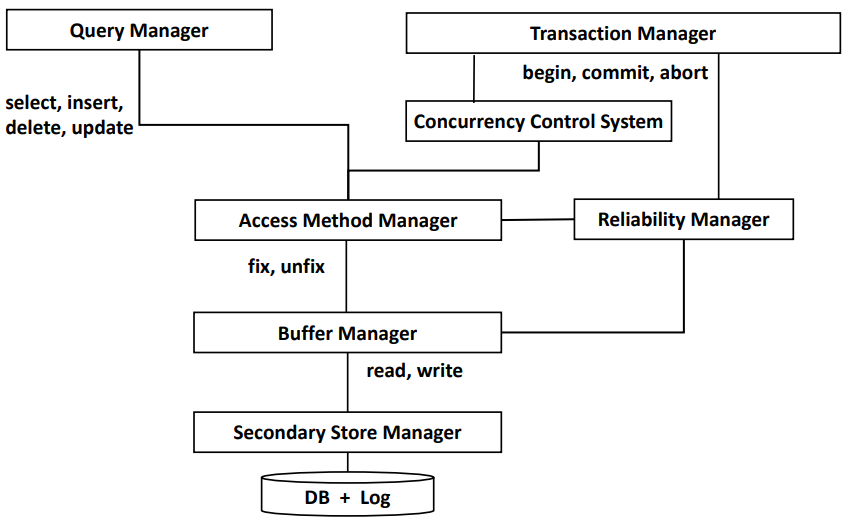
\includegraphics[width=0.75\linewidth]{images/architecture.png}
        \caption{Architecture of a Data Base Management System}
    \end{figure}

\newpage

\chapter{Concurrency}
    \section{Introduction}
    A DBMS usually needs to manage multiple applications. A unit of measurement used to evaluate the DBMS workload is the number of transaction per second (tps) handled by it. 
    To have an efficient usage of the database the DBMS needs to be able to handle concurrency while avoiding the insurgence of anomalies. 
    The concurrency control system schedules the order of the various transactions. 
    
    \section{Anomalies in concurrent transactions}
    The typical types on anomalies in concurrency are: 
    \begin{itemize}
        \item Lost update: an update is applied from a state that ignores a preceding update, which is lost.
            \begin{table}[H]
                \centering
                \begin{tabular}{c|c}
                \textbf{Transaction $t_1$}    & \textbf{Transaction $t_2$} \\ \hline
                $r_1(x)$                      &                            \\
                $x=x+1$                       &                            \\
                                              & $r_2(x)$                   \\
                                              & $x=x+1$                    \\
                                              & $w_2(x)$                   \\
                                              & commit                     \\
                $w_1(x)$                      &                            \\
                commit                        &                           
                \end{tabular}
            \end{table}
        \item Dirty read: an uncommitted value is used to update the data. 
            \begin{table}[H]
                \centering
                \begin{tabular}{c|c}
                \textbf{Transaction $t_1$} & \textbf{Transaction $t_2$} \\ \hline
                $r_1(x)$                   &                            \\
                $x=x+1$                    &                            \\
                $w_1(x)$                   &                            \\
                                        & $r_2(x)$                   \\
                                        & commit                     \\
                abort                      &                           
                \end{tabular}
            \end{table}
        \item Non-repeatable read: someone else updates a previously read value.
            \begin{table}[H]
                \centering
                \begin{tabular}{c|c}
                \textbf{Transaction $t_1$}  & \textbf{Transaction $t_2$} \\ \hline
                $r_1(x)$                    &                            \\
                                            & $r_2(x)$                   \\
                                            & $x=x+1$                    \\
                                            & $w_2(x)$                   \\
                                            & commit                     \\
                $r_1(x)$                    &                            \\
                commit                      & \multicolumn{1}{l}{}      
                \end{tabular}
            \end{table}
        \item Phantom update: someone else updates data that contributes to a previously valid constraint. 
            \begin{table}[H]
                \centering
                \begin{tabular}{c|c}
                \textbf{Transaction $t_1$} & \textbf{Transaction $t_2$} \\ \hline
                $r_1(x)$                   &                            \\
                                           & $r_2(y)$                   \\
                $r_1(y)$                   &                            \\
                                           & $y=y-100$                  \\
                                           & $r_2(z)$                   \\
                                           & $z=z+100$                  \\
                                           & $w_2(y)$                   \\
                                           & $w_2(z)$                   \\
                                           & commit                     \\
                $r_1(z)$                   &                            \\
                $s=x+y+z$                  &                            \\
                commit                     &                           
                \end{tabular}
            \end{table}
        \item Phantom insert: someone else inserts data that contributes to a previously read datum.
    \end{itemize}

    \section{Concurrency theory}
    \begin{definition}
        A \emph{model} is an abstraction of a system, object or process, which purposely disregards details to simplify the investigation of relevant properties. 
    \end{definition}
    Concurrency theory builds upon a model of transaction and concurrency control principles that help understanding the real systems. Real systems exploit implementation level 
    mechanisms (locks, snapshots) which help achieve some desirable properties postulated by the theory. 
    \begin{definition}
        An \emph{operation} consist in a reading or in a writing of a specific datum by a specific transaction. 
    \end{definition}
    \begin{definition}
        A \emph{schedule} is a sequence of operations performed by concurrent transactions that respects the order of operations of each transaction. 
    \end{definition}
    The transactions can be: serial, interleaved or nested. The number of serial schedules for $n$ transaction is equal to 
    \[N_S=n!\]
    while the total number of distinct schedules given the number of transaction $n$ is equal to: 
    \[N_D=\dfrac{\left( \sum_{i=1}^nk_i \right)!}{\prod_{i=1}^n \left( k_i! \right)}\]
    \begin{example}
        Given two transaction $T_1$ and $T_2$ we have six possible different schedules, where only two are serial:
        \begin{enumerate}
            \item $r_1(x) w_1(x) r_2(z) w2(z)$
            \item $r_2(z) w_2(z) r_1(x) w_1(x)$
            \item $r_1(x) r_2(z) w_1(x) w_2(z)$
            \item $r_2(z) r_1(x) w_2(z) w_1(x)$
            \item $r_1(x) r_2(z) w_2(z) w_1(x)$
            \item $r_2(z) r_1(x) w_1(x) w_2(z)$
        \end{enumerate}
        The first two are serial, the third and the fourth are nested, and the last two interleaved.
    \end{example}

    The concurrency control has to reject all the schedules that causes anomalies. 
    \begin{definition}
        The \emph{scheduler} is a component that accepts or rejects operations requested by the transactions. 
        The \emph{serial schedule} is a schedule in which the actions of each transaction occur in a contiguous sequence.
    \end{definition}
    A serializable schedule leaves the database in the same state as some serial schedule of the same transactions. This type of schedule is commonly accepted as a notion of schedule 
    correctness. To introduce the classes we have to initially make two assumptions: 
    \begin{itemize}
        \item The transactions are observed a posteriori. 
        \item The transactions limited to those that have been committed (commit-projection).
    \end{itemize}
    With the full schedule we can decide whether a schedule is admissible or not. In practice, the scheduler must take decisions while transaction are running because they cannot 
    know the sequence a priori.
    \section{View-serializability}
    \begin{definition}
        We say that:
        \begin{itemize}
            \item $r_i(x)$ \emph{reads-from} $w_j(x)$ when  $w_j(x)$  precedes  $r_i(x)$ and there is no  $w_k(x)$ in $S$ between  $r_i(x)$  and  $w_j(x)$. 
            \item  $w_i(x)$ in a schedule $S$ is a \emph{final write} if it is the last write on $x$ that occurs in $S$. 
        \end{itemize}
        Two schedules are said to be \emph{view-equivalent} ($S_i \approx_V S_j$) if they have:
        \begin{enumerate}
            \item The same operations. 
            \item The same reads-from relationships.
            \item The same final writes. 
        \end{enumerate}
    \end{definition}

    A schedule is view-serializable (VSR) if it is view-equivalent to a serial schedule of the same transactions.
    The reads-from relationship $r_i(x)$ reads-from $w_j(x)$ in a schedule $S$ assumes that $r_i(x)$ reads the value written by $w_j(x)$ independently of the time at which the 
    commit of $T_j$ occurs. In other words the value written by $w_j(x)$ could be uncommitted when $r_i(x)$ reads it, but we are sure (by definition of commit-projection) that it 
    will be committed.
    \begin{example}
        The following schedules are given:
        \begin{itemize}
            \item $S_1: w_0(x) r_2(x) r_1(x) w_2(x) w_2(z)$
            \item $S_2: w_0(x) r_1(x) r_2(x) w_2(x) w_2(z)$
            \item $S_3: w_0(x) r_1(x) w_1(x) r_2(x) w_1(z)$
            \item $S_4: w_0(x) r_1(x) w_1(x) w_1(z) r_2(x)$
            \item $S_5: r_1(x) r_2(x) w_1(x) w_2(x)$
            \item $S_6: r_1(x) r_2(x) w_2(x) r_1(x)$
            \item $S_7: r_1(x) r_1(y) r_2(z) r_2(y) w_2(y) w_2(z) r_1(z)$
        \end{itemize}
        We have that only $S_2$ and $S_3$ are serial. $S_1$ is view-equivalent to serial schedule $S_2$ (so it is view-serializable). 
        $S_3$ is not view-equivalent to $S_2$ (different operations) but is view-equivalent to serial schedule $S_4$, so it is also view-serializable. 

        $S_5$ corresponds to a lost update, $S_6$ corresponds to a non-repeatable read, and $S_7$ corresponds to a phantom update. All these schedules are non view-serializable. 
        
        The following schedules are given:
        \begin{itemize}
            \item $S_a: w_0(x) r_1(x) w_0(z) r_1(z) r_2(x) w_0(y) r_3(z) w_3(z) w_2(y) w_1(x) w_3(y)$
            \item $S_b: w_0(x) w_0(z) w_0(y) r_2(x) w_2(y) r_1(x) r_1(z) w_1(x) r_3(z) w_3(z) w_3(y)$
            \item $S_c: w_0(x) w_0(z) w_0(y) r_2(x) w_2(y) r_3(z) w_3(z) w_3(y) r_1(x) r_1(z) w_1(x)$
        \end{itemize}
        $S_a$ and $S_b$ are view-equivalent because all the reads-from relationship and final writes are the same. In fact, we have: 
        \begin{itemize}
            \item Reads-from: $r_1(x)$ from $w_0(x)$, $r_1(z)$ from $w_0(z)$, $r_2(x)$ from $w_0(x)$, $r_3(z)$ from $w_0(z)$.
            \item Final writes: $w_1(x)$, $w_3(y)$, $w_3(z)$.
        \end{itemize}
        $S_a$ and $S_c$ are not view-equivalent because not all the reads-from relationship are the same. 
    \end{example}
    Deciding view-equivalence of two given schedules is done in polynomial time and space. Deciding if a generic schedule is in VSR is an NP-complete problem. Therefore, we need to 
    find a stricter definition that is easier to check. The new definition may lead to rejecting some schedule that would be acceptable under view-serializability but not under the 
    stricter/faster criterion.
    
    \section{Conflict-serializability}
    \begin{definition}
        Two operations $o_i$ and $o_j$ ($i \neq j$) are in \emph{conflict} if they address the same resource and at least one of them is a write. There are tho possible cases:
    \end{definition}
    \begin{enumerate}
        \item Read-write conflicts ($r-w$ or $w-r$).
        \item Write-write conflicts ($w-w$).
    \end{enumerate}
    \begin{definition}
        Two schedules are \emph{conflict-equivalent} (($S_i \approx_C S_j$)) if $S_i$ and $S_j$ contain the same operations and in all the conflicting pairs the transactions occur in the same order. 
        A schedule is \emph{conflict-serializable} (CSR) if and only if it is conflict equivalent to a serial schedule of the same transactions. 
    \end{definition}
    We have that $VSR \subset CSR$: all conflict-serializable schedules are also view- serializable, but the inverse is not necessarily true.
    So, we have that conflict-equivalence implies view-equivalence. 
    \begin{proof}[VSR is a subset of CSR]
        Schedule $S = r_1(x) w_2(x) w_1(x) w_3(x)$ is: 
        \begin{itemize}
            \item View-serializable.
            \item Not conflict-serializable
        \end{itemize}
        It is possible to check that there is no conflict-equivalent serial schedule.
    \end{proof}
    \begin{proof}[CSR implies VSR]
        We assume $S_1 \approx_C S_2$ and prove that $S_1 \approx_V S_2$. $S_1$ and $S_2$ must have: 
        \begin{itemize}
            \item The same final writes: if they didn't, there would be at least two writes in a different order, and since two
                writes are conflicting operations, the schedules would not be $\approx_C$. 
            \item The same reads-from relations: if not, there would be at least one pair of conflicting operations in a different
                order, and therefore, again, $\approx_C$ would be violated. 
        \end{itemize}
    \end{proof}
    The testing of view-serializability is done with a conflict graph that has one node for each transaction $T_i$, and one arc from $T_i$ to $T_j$ if there exists at least one conflict between an operation $o_i$ of $T_i$ and an operation $o_j$ of $T_j$ such that $o_i$ precedes $o_j$.
    \begin{theorem}
        A schedule is in CSR if and only if its conflict graph is acyclic.
    \end{theorem}
    \begin{example}
        We are given the schedule \[S: w_0(x) r_1(x) w_0(z) r_1(z) r_2(x) w_0(y) r_3(z) w_3(z) w_2(y) w_1(x) w_3(y)\]
        To test the conflict serializability we have to do the following steps: 
        \begin{enumerate}
            \item Create all the nodes based on the number of transactions of the schedule. 
            \item Divide the operation based on resource requested.
            \item Check all the write-write and read-write relationships in each subset, and add the arcs based on these. 
        \end{enumerate}
        In the given example we obtain: 
        \begin{itemize}
            \item $x: w_0 r_1 r_2 w_1$
            \item $y: w_0 w_2 w_3$
            \item $z: w_0 r_1 r_3 w_3$
        \end{itemize}
        \begin{figure}[H]
            \centering
            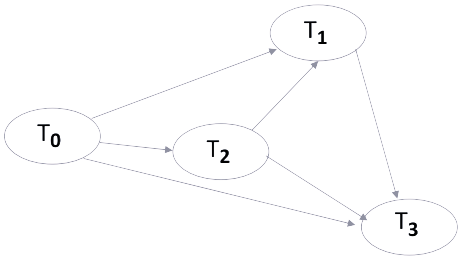
\includegraphics[width=0.5\linewidth]{images/conflict.png}
        \end{figure}
    \end{example}
    \begin{proof}[CSR implies acyclicity of the conflict graph]
        Consider a schedule $S$ in $CSR$. As such, it is $\approx_C$ to a serial schedule. 
        Without loss of generality we can label the transactions of $S$ to say that their order in the serial schedule is: $T_1 T_2 \dots T_n$.
        Since the serial schedule has all conflicting pairs in the same order as schedule $S$, in the conflict graph there can only be arcs $(i,j)$, with $i<j$. 
        Then the graph is acyclic, as a cycle requires at least an arc $(i,j)$ with $i>j$.
    \end{proof}
    \begin{proof}[Acyclicity of the conflict graph implies CSR]
        If $S$'s graph is acyclic then it induces a topological (partial) ordering on its nodes. The same partial order exists on the transactions of $S$. 
        Any serial schedule whose transactions are ordered according to the partial order is conflict-equivalent to $S$, because for all conflicting pairs $(i,j)$ it is always $i<j$. 
    \end{proof}
        
    \section{Concurrency control in practice}
    CSR checking would be efficient if we knew the graph from the beginning, but usually we don't. Therefore, a scheduler must rather work online. So, it is not feasible to maintain the conflict graph, update it, and check its acyclicity at each operation request. At the same time, the assumption that concurrency control can work only with the commit-projection of the schedule is unrealistic because aborts do occur. We need some simple on-line decision criterion for the scheduler, which must avoid as many anomalies as possible, and have negligible overhead. 
        
    When dealing with online concurrency control, it is important also to consider arrival sequences. The CC system maps an arrival sequence into an effective a posteriori schedule. To implement this on-line scheduling we use two main families of techniques:
    \begin{itemize}
        \item Pessimistic (locks): if a resource is taken, make the requester wait or pre-empt the holder.
        \item Optimistic (timestamps and versions): serve as many requests as possible, possibly using out-of-date versions of the data. 
    \end{itemize}
    Usually, commercial systems take the best of both worlds. 

    
    \section{Locking}




    
\end{document}